Heterogeneous computer systems, such as traditional CPU-GPU based systems, 
% keep it simple and remove:
% require different programming models for
% different execution unit types, and they often 
often expose disjoint memory spaces to the programmer,
such as main memory and device memory, with the need
to explicitly transfer data between these.
% \TODO{I was confused with the next 3 sentecnes , please check this version}
The different memories usually 
require different memory access operations and
different pointer types. % on CPU and accelerator side.
% Done, removed the rest as it might confuse:   even in programming
% environments where a single-source program
% involves both CPU and accelerator code.
Also, encoding memory transfers as message passing communications
leads to low-level code that is more error-prone. 
% While the former problem is often solved by 
% compiler support (as in OpenACC, OpenMP4.5 and
% domain-specific languages)
% or other high-level programming
% abstractions (e.g.\ skeleton programming as in 
% SkePU or SkelCL), e.g. 
A commonly used software technique to abstract away the
distributed memory, the explicit message passing,
and the asymmetric memory access mechanisms
consists in providing the programmer with an 
object-based shared memory emulation. For CPU-GPU systems,
this can be done in the form of special data-containers,
which are generic, STL-like data abstractions such as 
\verb+vector<...>+ that 
% \TODO{I am a bit confused with the ``wrap aggregate''} 
% is multi-element better?
wrap multi-element data structures such as arrays. These 
data-container objects
 internally perform transparent, coherent
software caching
of (subsets of) accessed elements in the different memories 
so they can be reused (as long as not invalidated) 
in order to
avoid unnecessary data transfers. Such data-containers 
(sometimes also referred to as ''smart'' containers as they can
transparently perform data transfer and memory allocation optimizations
\cite{Dastgeer-IJPP15}) 
are provided in a number of programming frameworks 
for heterogeneous systems, such as
StarPU \cite{StarPU} and SkePU \cite{Enmyren10,Dastgeer-IJPP15}. StarPU is a 
C-based library that provides API functions to
define multi-variant tasks for dynamic scheduling
where the data containers are used for modeling 
the operand data-flow
among the dynamically scheduled tasks. 
SkePU defines device-independent 
multi-backend skeletons like map, reduce,
scan, stencil etc.\ where operands are
passed to skeleton calls within data containers.

VectorPU \cite{VectorPU-2017} is a recent C++-only
open-source
programming framework for CPU-GPU heterogeneous systems. 
VectorPU relies on the specification of 
\textit{components}, which are functions that contain kernels for execution
on either CPU or GPU. Programming in VectorPU is thus not restricted 
to using predefined skeletons like SkePU, 
but leads to more high-level and more concise code than StarPU. 
Like StarPU, VectorPU requires the programmer
to annotate each operand of a component
%\TODO{passed to components? (I find the ``operand'' a bit abrupt here)} 
with the access mode (read, write, or both) including the 
accessing unit (CPU, GPU), and uses smart data containers for automatic transparent
software caching based on this access mode information.

The implementation of VectorPU makes excessive use of static metaprogramming; this provides a light-weight realization of the access mode annotations and of the software caching, 
which only require a standard C++ compiler. Emulating these 
light-weight
component and access mode constructs without additional language
and compiler support (in contrast to, e.g., OpenACC or OpenMP), 
leads however to some compromises in static analyzability.
In particular, VectorPU has no explicit type system for the
access modes, as these are not known to the C++ compiler.

In this paper, we investigate how to formalize access modes
and data transfers in CPU-GPU heterogeneous systems and prove 
the correctness of the software
cache coherence mechanism used in VectorPU.
The contributions of this paper are:

\begin{itemize}
\item We introduce a simple effect system modeling the semantics of memory
   accesses and communication in a CPU-GPU heterogeneous system,
   and define a small calculus expressing different memory
   accesses and their composition across program traces. 
\item We express VectorPU operations as higher-level statements
    that can be translated into the core calculus,
    and show that, if all memory accesses are performed 
    through VectorPU operations, the memory cannot reach an 
    inconsistent state and all memory accesses succeed.
\end{itemize}

This paper is organized as follows:
Section~\ref{VectorPU} reviews VectorPU as far as required for  this paper, for further information we refer to \cite{VectorPU-2017}.
Section~\ref{sec:Formal} provides our formalization of VectorPU programs and
their semantics, and proves that the coherence mechanism used in
VectorPU is sound. Section~\ref{sec:RW} discusses related work, and 
Section~\ref{sec:conclusion} concludes.

\begin{figure}
\begin{center}
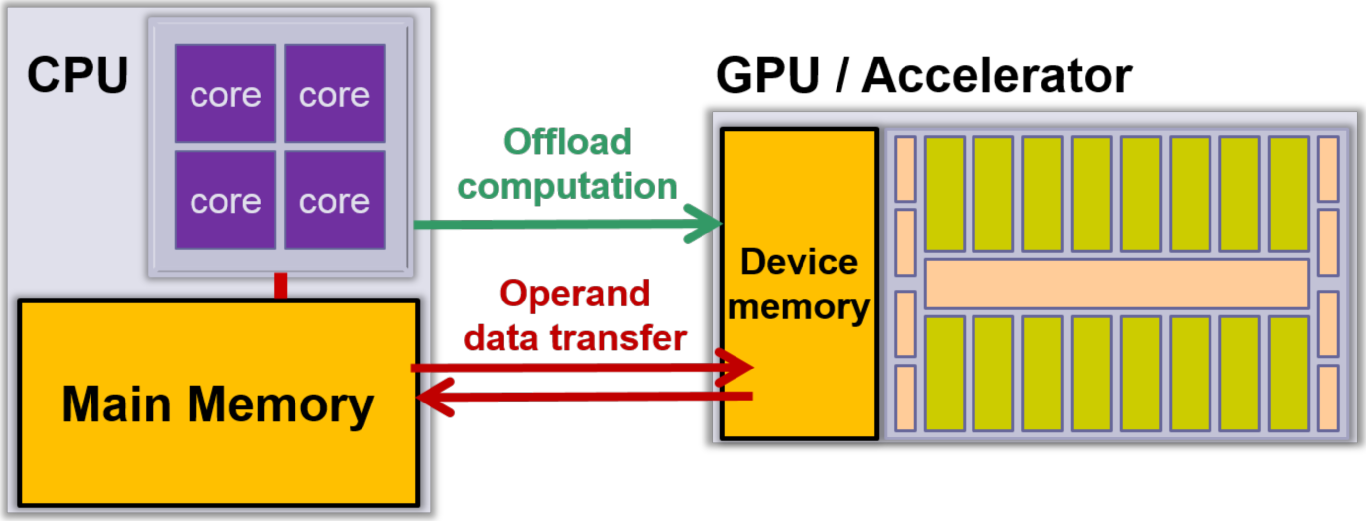
\includegraphics[width=0.58\textwidth]{img/CPU-GPU.png}
\caption{\label{fig:CPU-GPU}A GPU-based system with distributed address space}
\end{center}
\vspace{-3ex}
\end{figure}

\section{VectorPU}\label{VectorPU}

In heterogeneous systems with separate address spaces, for example in 
many GPU-based systems, a general-purpose processor
(CPU) with direct access to main memory is connected by some network
(e.g., PCIe bus) to one or several accelerators
(e.g., GPUs) each having its own device memory,
see Figure~\ref{fig:CPU-GPU}. Native programming models
for such systems such as CUDA typically expose the distributed address spaces to the programmer, who has to write explicit 
code for data transfers and device memory management.
Often, programs for such systems even must be organized in multiple source files
as different programming models and different toolchains
are to be used for different types of execution unit.
This enforces a low-level programming style. 
Accordingly, a number of single-source 
programming approaches have been proposed that abstract away the distribution 
by providing a virtual shared address space. Examples include directive-based
language extensions such as OpenACC and OpenMP4.5, and C++-only approaches 
such as the library-based skeleton programming framework SkePU \cite{Dastgeer-IJPP15}
and the recent macro-based framework \textit{VectorPU}, 
which we focus on in this paper as a case study.

\textit{VectorPU} \cite{VectorPU-2017} is an open-source\footnote{http://www.ida.liu.se/labs/pelab/vectorpu, https://github.com/lilu09/vectorpu} lightweight C++-only 
high-level programming layer
for writing single-source heterogeneous programs for Nvidia CUDA GPU-based systems.

Aggregate operand data structures 
passed into or out of  function calls are
to be wrapped by special data containers known to VectorPU.
VectorPU currently provides one generic data container,
called \verb+vector<...>+,
with multiple variants that 
eliminate the overhead of managing heterogeneity and distribution when not required (e.g., when no GPU is available). 
\verb+vector<...>+ inherits functionality from STL \verb.vector. 
and from Nvidia Thrust \verb.vector., and
wraps a C++ array allocated in main memory. 
VectorPU automatically creates on demand
copies of to-be accessed elements in device memory and keeps all copies coherent using
a simple coherence protocol, data transfers are only performed when needed. 

VectorPU programs are organized as a set of C++ functions, some of which
might internally use device-specific programming CUDA constructs\footnote{%
VectorPU allows to directly annotate a CUDA kernel function, in addition to annotating its C++ wrapper function.} while others
are expected to execute on the host, using one or possibly multiple cores.
VectorPU \emph{components} are functions that are supposed to contain (CPU or device)
kernel functionality and for which  operands are passed as VectorPU data container objects. 
Components and the types of execution units that
access their operands are implicitly marked 
by annotating the operands of the function, either at a call of the function
or for the formal parameters in the function's declaration, 
with VectorPU \emph{access mode specifiers}.%
\footnote{In contrast to e.g.\ SkePU \cite{Enmyren10} which overloads element
access and iterator operations so that monitored 
accesses are also possible on demand in non-componentized (i.e., 
ordinary C++) CPU code,
VectorPU only relies on access mode annotations 
to perform lazy data transfer,
not knowing when data is going to be accessed inside a component.}
% however, SkePU knows by overloading element accesses.
% By overloading element
% access and iterator operations, 

The access mode specifiers,
such as \texttt{R} (read on CPU), \texttt{W} (write on CPU), \texttt{RW} 
(update, i.e., both read and write, on CPU), \texttt{GR} (read on GPU) and so forth,
are available both as annotations of function signatures%
\footnote{The current VectorPU prototype implementation does not
(yet) type-check access-mode annotations in signatures of externally defined functions.} and
as C++ preprocessor macros that expand at compilation into (possibly, device-specific) C++ pointer
expressions and side effects that allow to generate device specific access code
and use device-specific pointer types for the chosen execution unit. 
For instance, \texttt{GW(x)} expands to a GPU pointer to
the GPU device copy of \texttt{x},
which might be dereferenced for GPU writing accesses to \texttt{x},
such as the GPU code: \verb:*( GW(x) + 2 ) = 3.14:.
\texttt{GWI(x)} evaluates to an Thrust-compatible iterator onto the 
GPU device copy of \texttt{x}, and \texttt{WEI(x)} to an iterator-end reference
to the last element of \texttt{x} on CPU side.
%
It is also possible to specify partial access of a \verb:vector:
% that expand into pointers to the first and last element
% of an interval of elements to be accessed, 
instead of the
entire \verb.vector. data structure\footnote{The current
VectorPU implementation does not (yet) support coherence for 
\emph{overlapping}
intervals of elements resulting from multiple (partial) accesses
some of which (may) access the same element.
A solution for this problem has been described for SkePU
smart containers by Dastgeer~\cite{Dastgeer-IJPP15}.}.
%
Table~\ref{tab:modes} summarizes the access mode annotations
currently defined for VectorPU.

\begin{table}
\caption{\label{tab:modes}VectorPU access mode annotations for a parameter  \cite{VectorPU-2017}}

\begin{center}
\begin{tabular}{|lll|}
\hline
Access Mode & On Host & On Device \\
\hline
Read pointer & \texttt{R} & \texttt{GR} \\
Write pointer & \texttt{W} & \texttt{GW} \\
Read and Write pointer & \texttt{RW} & \texttt{GRW} \\
Read Iterator & \texttt{RI} & \texttt{GRI} \\
Read End Iterator & \texttt{REI} & \texttt{GREI}\\
Write Iterator & \texttt{WI} & \texttt{GWI}\\
Write End Iterator & \texttt{WEI} & \texttt{GWEI}\\
Read and Write Iterator & \texttt{RWI} & \texttt{GRWI}\\
Read and Write End Iterator & \texttt{RWEI} & \texttt{GRWEI}\\
Not Applicable & \texttt{NA} & \texttt{NA} \\
\hline
\end{tabular}
\vspace{-3ex}
\end{center}
\end{table}


The following example (adapted from \cite{VectorPU-2017}) 
of a CUDA kernel wrapped in an 
 annotated function \verb.bar. shows the use of 
VectorPU access mode annotations at function declaration:

{\footnotesize \begin{verbatim}
// Example (annotations at function declaration): 
__global__
void bar ( const float *x [[GR]], float *y [[GW]],
                 float *z [[GRW]], int size )
{ ... CUDA kernel code ... }
\end{verbatim}}

Here, the operand array pointed to by \verb.x. may be read (only) by the GPU within \verb.bar.,
operand array \verb.y. may be written (only) by the GPU, and 
operand array \verb.z. may be read or written (or both) by the GPU.
When calling \verb.bar., the
first three operands need to be passed as VectorPU \verb.vector. 
container objects.
The \verb.size. formal parameter is a scalar (not a data container), so it
will be available on GPU on a copy-in basis but no coherence will
be provided for it by VectorPU.

It is also possible to put the annotations into a call, and hence characterize a function as a VectorPU component:


{\footnotesize \begin{verbatim}
// declare a CPU function:
void foo ( const float *x, float *y,
            float *z, int size );

// declare three vectors:
vectorpu::vector<float> vx(100), vy(100), vz(100);

// call to VectorPU annotated function foo:
foo ( R( vx ), W( vy ), RW( vz ), size ) ;
\end{verbatim}}

Here, the access mode specifiers and the resulting coherence policy
 only apply to that particular invocation of \verb-foo-, while other
invocations of \verb-foo- might use different access mode specifiers.
The following example shows how to use iterators:

{\footnotesize \begin{verbatim}
vectorpu::vector<My_Type> vx(N);
std::generate( WI(vx), WEI(vx), RandomNumber );
thrust::sort( GRWI(vx), GRWEI(vx));
std::copy( RI(vx), REI(vx),
           ostream_iterator<My_Type>(cout, ""));
\end{verbatim}}

\noindent 
where \verb.std::generate. is a CPU function filling a section between
two addresses with values (here, random numbers),
and \verb.thrust::sort. denotes the GPU sorting functionality.
provided by the Nvidia Thrust library. 

\begin{figure}
\begin{small}
\begin{verbatim}
void coherent_on_cpu_r(){
  	 if( !cpu_coherent_unit ){
  		 download();
  		 cpu_coherent_unit=true;
  	 }
}
void coherent_on_cpu_w(){
  	 cpu_coherent_unit=true;
  	 gpu_coherent_unit=false;
}
void coherent_on_cpu_rw(){
  	 if( !cpu_coherent_unit ){
  		 download();
  		 cpu_coherent_unit=true;
  	 }
  	 gpu_coherent_unit=false;
}
void coherent_on_gpu_r(){
  	 if( !gpu_coherent_unit ){
  		 upload();
  		 gpu_coherent_unit=true;
	 }
}
void coherent_on_gpu_w(){
  	 gpu_coherent_unit=true;
  	 cpu_coherent_unit=false;
}
void coherent_on_gpu_rw(){
  	 if( !gpu_coherent_unit ){
  		 upload();
  		 gpu_coherent_unit=true;
  	 }
  	 cpu_coherent_unit=false;
}
\end{verbatim}
\end{small}
\caption{\label{fig:vectorpucoherence}Coherence control code,i
    here for simple vectors,
    in \texttt{vectorpu.h}. Functions \texttt{download} and
    \texttt{upload} are implemented using CUDA
    \texttt{thrust::copy}. Validity of copies on CPU and GPU
     is indicated
     by the flags \texttt{cpu\_coherent\_unit} and
     \texttt{gpu\_coherent\_unit} respectively; both are
     initialized to \texttt{true}
     in code allocating new vectors (not shown).}
     % 
     % for the records:
     %
     % template <class T, class Index_Type=std::size_t>
     % struct min_vector : public std::vector<T>, public thrust::device_vector<T> {
     % explicit min_vector(Index_Type _array_size):
     %  	 std::vector<T>::vector(_array_size),
     %  	 thrust::device_vector<T>::device_vector(_array_size),
	 % cpu_coherent_unit(true),
	 % gpu_coherent_unit(true),
     %  	 array_size(_array_size),
     % start_pos(0) {}
\end{figure}

\vspace{1.4mm}
\noindent
\textit{Implementation notes }
In the source code of VectorPU, the code
relevant for our work is the part of \verb+vectorpu.h+%
\footnote{The VectorPU source code can be found at
\texttt{https://github.com/lilu09/vectorpu}.} 
that handles coherence. Its implementation for the various
variants of \texttt{vector} 
(see the code excerpt in Fig.~\ref{fig:vectorpucoherence} for
simple \texttt{vector}s) follows a
simple valid-invalid protocol.
%(single-reader single-writer sharing).

\vspace{1.4mm}
\noindent
\textit{Efficiency }
Using only available C++(11) language features, 
VectorPU provides a flexible unified memory
view where all data transfer and device memory management
is abstracted away from the programmer. Nevertheless,
its efficiency is on par with that of handwritten CUDA code
containing explicit data movement and memory management code
\cite{VectorPU-2017}.
In particular, the VectorPU prototype was shown to
achieve 1.4x to 13.29x speedup over good quality
code using Nvidia's \textit{Unified Memory} API
on several machines ranging from laptops to supercomputer nodes,
with Kepler and Maxwell GPUs. For a further discussion of
VectorPU features, such as
specialized versions of \verb-vector-, for descriptions
of how to use VectorPU together with lambda expressions 
e.g.\ to express skeleton computations, and for further
experimental results 
we refer to \cite{VectorPU-2017}.
